%% ----------------------------------------------------------------
%% Appendix: Validation and verification of the in-house solver
%% ----------------------------------------------------------------
%!TeX root = subfile
\label{chapter:appendixB}
\markboth{Appendix B Validation and verification of the in-house solver}{Appendix B Validation and verification of the in-house solver}
\documentclass[../main.tex]{subfiles}
% ---------------------------------------------------------------- 
\begin{document}
A grid convergence study has been conducted in order verify the correct implementation of the governing equations and to show that the selected grid resolution and averaging time length is suitable for a proper analysis.
Three grids with different resolution $(\Delta)$ designed as shown in \fref{fig:computational_domain} have been investigated for the $L_z=\pi$ case (see details in \tref{tab:verification_grids}).
The refinement ratio is $\sqrt{2}$.

\begin{figure}
  \centerline{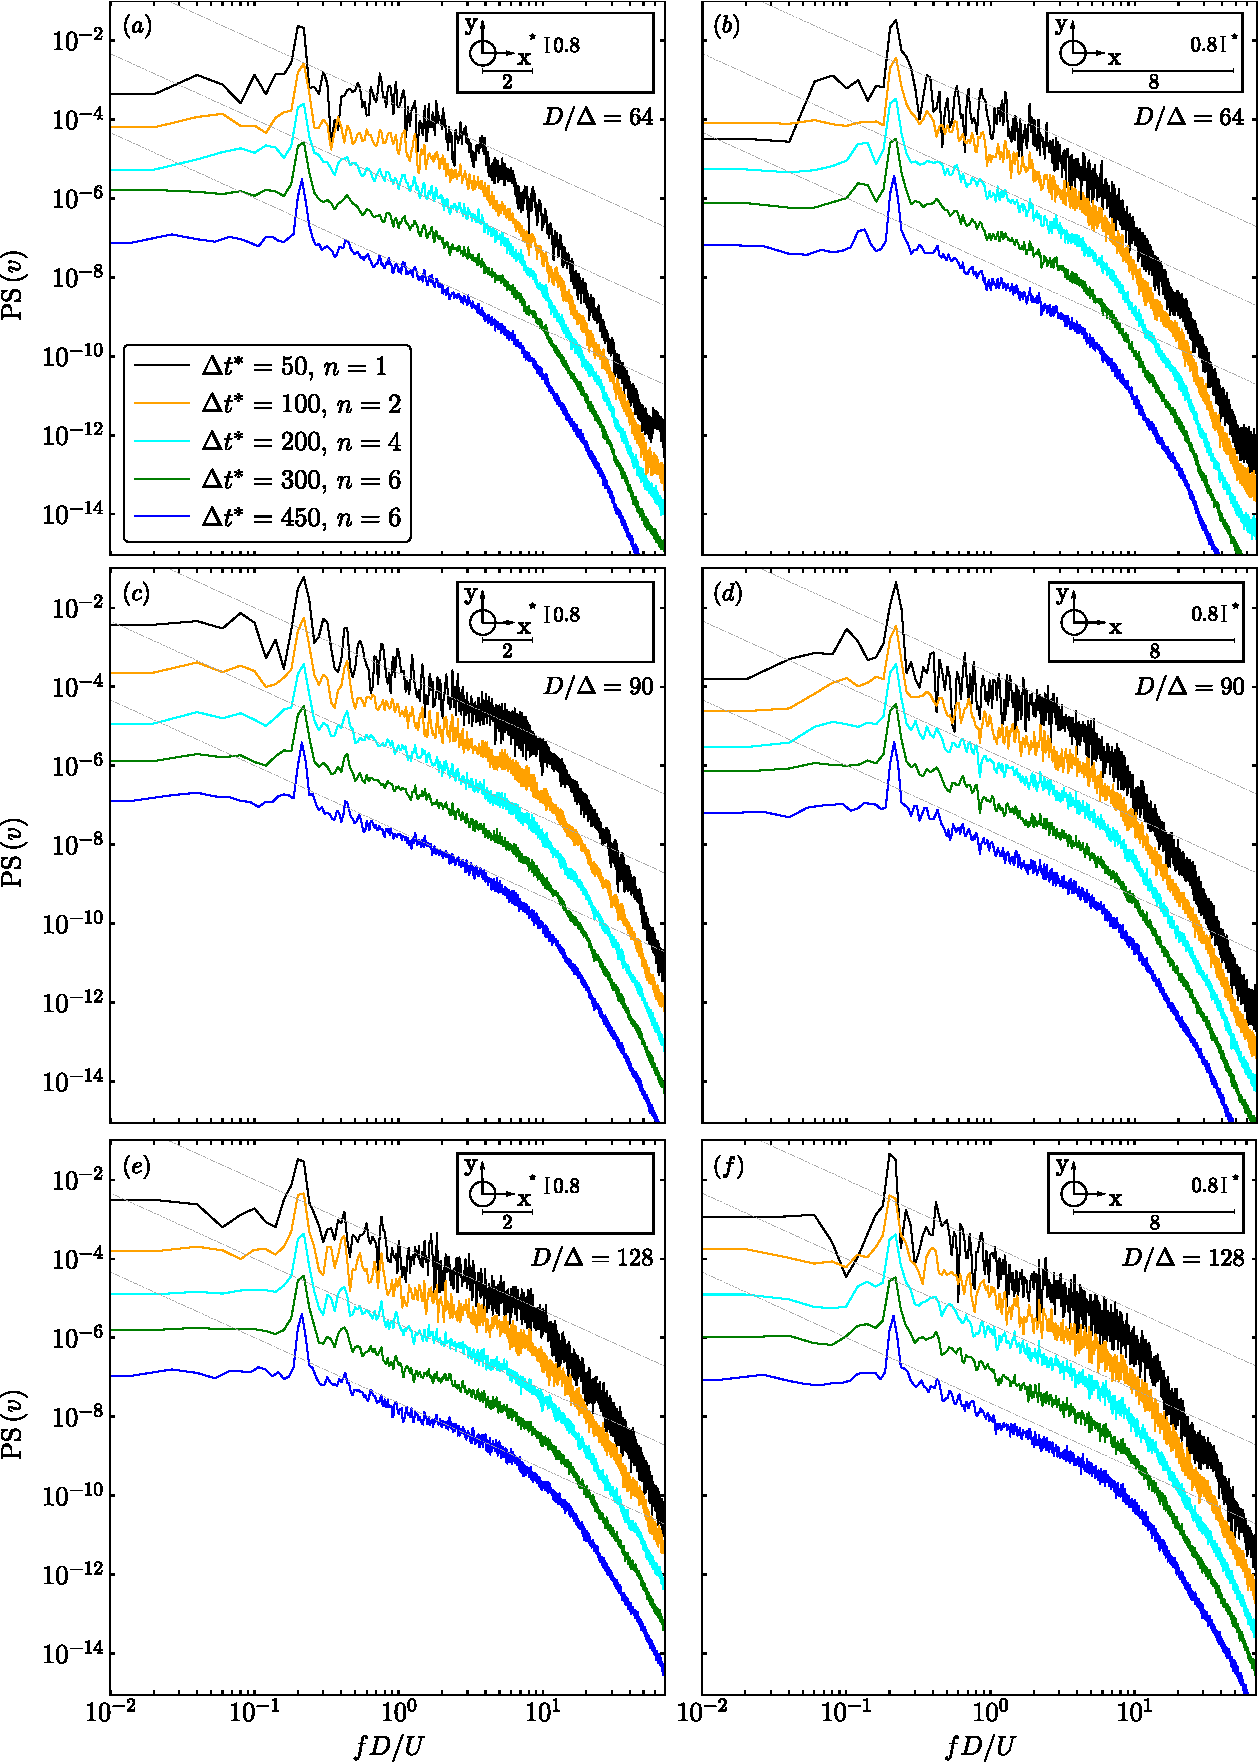
\includegraphics[width=0.94\textwidth]{appendixB/fig10}}
  \caption{Vertical velocity component temporal PS at the close (left) and far (right) wake regions.
The coarse, medium and fine grid results are displayed at the first, second and third row respectively.
The spectra are shifted a factor of 10 and the vertical axis ticks correspond to the $\Delta t^*=50$ case.
The number of the time signal splits selected for the Welch method ($n$) ensures a minimum of $\Delta t^*=50$ per split (at least 8 times larger than the lowest frequency of interest, i.e. the shedding frequency which is approximately $\Delta t^*=5$), and a maximum of 6 splits per total time signal.
The dotted line corresponds to a $-5/3$ slope.}
\label{fig:velocity_spectras_GC}
\end{figure}

\begin{figure}
  \centerline{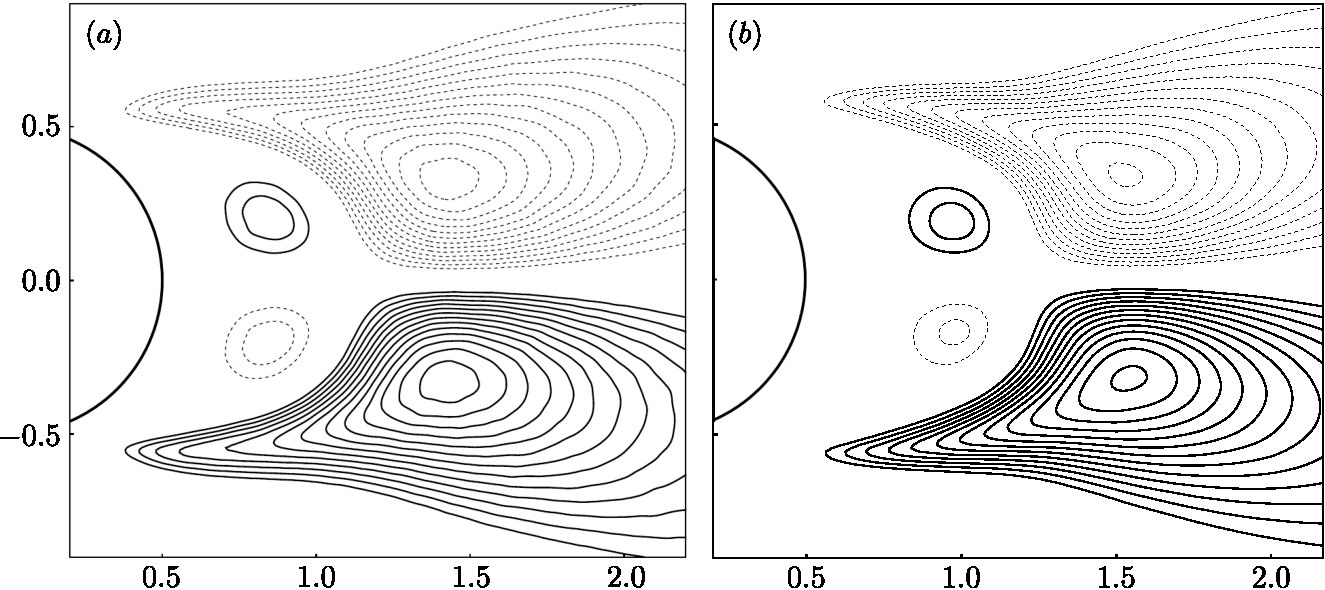
\includegraphics[width=1\textwidth]{appendixB/fig11}}
  \caption{Comparison of the Reynolds shear stress $\overline{u'v'}$ between: (a) DNS data from \cite{Dong2005} and (b) present solver.
The contour levels criteria is the same as the reference data: ${|\overline{u'v'}|}_{\mathrm{min}}=0.03$ and $\Delta\overline{u'v'}=0.01$.
Positive and negative levels are noted with continuous and dashed lines respectively.}
\label{fig:uv_validation}
\end{figure}

The quantities of interest of the present work are the turbulence statistics arising from time and spatial averages.
Because of this, we need to ensure that the presented results are statistically stationary and have converged in spatial resolution terms.
The velocity temporal power spectrum constructed analogously to \fref{fig:velocity_spectras} at the $(x,y)=\left(2,0.8\right),\left(8,0.8\right)$ locations is used with this purpose.
The spectrum produced by the investigated grids is shown for different time signal lengths in \fref{fig:velocity_spectras_GC}.

\begin{table}
  \begin{center}
\def~{\hphantom{0}}
  \begin{tabular}{rrr}
  	   \toprule
       $D/\Delta$ & $N_{CG}$ (M) & $N_{T}$ (M) \\[3pt]
       \midrule
       64  & 65.3 & 109.2\\
       90  & 189.5 & 311.4 \\
       128 & 510.6 & 855.6\\
       \bottomrule
  \end{tabular}
  \caption{Details of the three different grids ranging from coarse ($D/\Delta=64$, i.e. 64 cells per diameter) to fine ($D/\Delta=128)$ for $L_z=\pi$.
$N_{GC}$ refers to the total number of cells (in millions) for the Cartesian grid subdomain.
$N_T$ refers to the total number of cells (in millions).}
  \label{tab:verification_grids}
  \end{center}
\end{table}

At the near wake region, the coarse grid shows a converged spectrum ($-5/3$ inertial subrange decay) for time signals with $\Delta t^*>200$.
A similar behaviour is captured with the medium grid, which shows a converged spectrum for time signals with $\Delta t^*>100$ and the resulting inertial subrange accommodates more frequencies.
At the far wake region, the coarse grid presents slightly steeper spectra than at the close wake region.
This can be caused by an insufficient resolution in span, which would induce a two-dimensionalisation effect.
On the other hand, the medium grid still presents converged spectra for time signals with $\Delta t^*>100$.
The fine grid leads to results very similar to the medium grid.
Hence, it is shown that using the medium grid with simulation times over $\Delta t^*>100$ provides statistically stationary results both in the close and far wake regions ($\Delta t^*=500$ is used in the results presented in \cref{chapter:jfm2019}).

To validate the wake turbulence statistics, the Reynolds shear stress $\overline{u'v'}$ has also been qualitatively analysed.
It can be observed in \fref{fig:uv_validation} that the shear stress predicted by the present solver is in very good agreement with the DNS data from \cite{Dong2005}, with just a slight shift of the field structures on the streamwise direction.
All positive and negative regions are correctly captured which display an antisymmetric pattern with respect to the centreline of the wake.
% ---------------------------------------------------------------- 
\end{document}